% #############################################################################
% This is Chapter 7 - Implementation
% !TEX root = ../main.tex
% #############################################################################
% SOURCE: docs/framework/Apex-Implementation-Report.docx is the authoritative
% grounding for this chapter (architecture, testing, deployment, incident log).
% Figures come from docs/diagrams/architecture-a.puml, architecture-b.puml and
% user-flow-a.puml / user-flow-b.puml. The architecture figure is authored as two
% separate sources (a decomposition, not a crop of one wide rendering): part one
% collapses the guarded egress layer to a single component, part two expands it.
% Dashed violet stubs carry every connector that crosses between the two halves.
% Suite sizes are a snapshot and are stated as such in the text.
% #############################################################################
% Title changed 2026-09-14 (supervisor feedback + Tomás): plainer, paired
% with Chapter 6's "Research Proposal" title rather than naming the product.
\fancychapter{Implementation}
\label{chap:apex}

The framework presented in \Cref{chap:proposal} describes a methodology. This chapter presents Apex, the working software system instantiating it, which serves both as evidence that the framework's governance constructs are implementable and as the vehicle through which the framework is demonstrated and evaluated in \Cref{chap:demonstration,chap:evaluation}. In \ac{DSRM} terms the two are distinct artefacts produced by the same Design and Development activity: a method and its instantiation. The chapter answers \ac{DRQ}3, and answering it honestly means reporting which constructs resisted implementation as well as which did not.

% #############################################################################
\section{Purpose and Positioning}
\label{sec:apex_purpose}

% The distinction below is the one that most needs stating early and plainly:
% Apex is not competing with coding agents on convenience.

Apex is not a coding agent and is not positioned against one. A coding agent accelerates the writing of code; Apex governs whether the code that results still answers the question that prompted it. The two are complementary, and the distinction is the whole reason the system exists: acceleration without anchoring is the condition \Cref{chap:intro} shows moves the bottleneck to review rather than removing it. Every artefact Apex produces carries a stable specification identifier back to the requirement it derives from, so divergence between what was agreed and what was built becomes a detectable event rather than a drift nobody is positioned to notice.

What Apex deliberately does not do is as much part of its definition. It does not train or fine-tune models, and treats the model as a third-party capability that may change beneath it. It does not provision infrastructure: where a release needs configuration or migration scripts it generates them for a human or a \ac{CI} pipeline to execute, and never applies them itself. And it does not replace the project management tool a team already uses. It sits above that tool, reads and writes through it, and expects the team's existing board to remain the system of record for work items, which is why the framework's board guidance in \Cref{sec:work_organisation} asks only that a team's own columns map onto framework phases rather than that they be renamed.

% #############################################################################
\section{Architecture}
\label{sec:apex_architecture}

Apex is a split full-stack application. The frontend is Next.js 15 with the App Router in TypeScript; the backend is Python 3.12 with FastAPI; the two communicate over a typed REST API. Server state on the frontend is owned by React Query and client state by Zustand, with credentials persisted only to session storage so that they clear when the tab closes. Backend routers are kept deliberately thin, with workflow logic held in a service layer and a schema for every request and response boundary. That separation is an engineering choice rather than an accident of growth: it keeps route handlers testable as thin adapters and workflow logic testable in isolation from \ac{HTTP} concerns, which is what made the test strategy in \Cref{sec:apex_qa} possible at the sizes it reaches. \Cref{fig:apex_architecture,fig:apex_architecture_b} show the arrangement.

\begin{figure}[htbp]
    \centering
    
\includegraphics[width=\linewidth]{./Images/architecture-a.png}
    \caption[Apex's system architecture, part one of two]{Apex's system architecture, part one of two: the frontend, the backend and the specification store. The figure is split across two pages for legibility; the point of it is the position of two boundaries rather than the inventory of components, and this half shows the first, where all workflow state is written to a per-tenant, per-project specification store rather than to an application database. The backend's guarded egress layer is drawn collapsed to a single component here and expanded in \Cref{fig:apex_architecture_b}; the dashed connector on the right marks where the two halves join.}
    \label{fig:apex_architecture}
\end{figure}

Five properties of that architecture carry framework constructs rather than merely supporting them:

\begin{itemize}[leftmargin=0.6cm, itemsep=0.5em]

\item \textbf{Spec-anchored storage.} All workflow state lives in Markdown context files plus a machine-readable story index, under a path keyed first by instance then by project, so a hosted account and a private deployment of the same tool stay separate tenants for the same user. Storage abstracts over local disk or cloud file storage on one code path, verified by the test suite pinning it to local disk rather than a stand-in. This is Spec-Anchored Continuity made concrete: files that outlive any session, accessed only through a single service, never a direct import, since that service is where per-request project isolation is enforced (\Cref{sec:apex_qa}).

\item \textbf{A deliberate single-writer concurrency model.} The backend was originally pinned to one replica and one worker: the story index and workspace configuration live on shared file storage guarded only by a process-local lock, so a second replica would silently race on writes rather than crash, and a lost update looks like success. This was a documented constraint with a stated precondition for lifting it, subsequently built and enabled: an optional coordination layer promotes the locks to cross-replica equivalents when configured, falling back to byte-identical single-replica behaviour otherwise. Running in production with three replicas since June 2026, verified via live client connections.

\item \textbf{Proxy-first external integration.} Every outbound call to a user-configurable host is proxied server-side, closing server-side request forgery: the proxy validates \ac{HTTPS} and a non-private address before forwarding, and caps relayed body size. The identity anchor a request is validated against derives from the same validated host, which is what makes the storage isolation above trustworthy. One integration is a deliberate browser-direct exception whose credential never reaches the backend; two operations within it are not exceptions, needing a server-side filesystem and a server-held credential respectively.

\item \textbf{The project management adapter.} Apex reads and writes a board the team already has rather than owning one, through a single adapter interface, built against Taiga first with Jira and Plane added behind the same interface (Plane specifically because it is the tool the partner organisation in \Cref{chap:demonstration} is moving to). Adding a second and third tool tested \Cref{sec:framework_scope}'s claim that tool-independence is a property a mechanism must have, not one the product provides: it held at the level of operations (differing authentication shapes and identifier types both absorbed by generalising the identity anchor and minting a synthetic identifier) but not at the level of guarantees, since three of the second tool's \ac{API} limitations, no page update or delete endpoint, no optimistic-concurrency field, no server-side label filter, are permanent, each only mitigated at application level rather than fixed.

\item \textbf{Provider abstraction.} The model provider is detected from the model identifier and routed accordingly, with provider errors mapped to typed exceptions at a single boundary so no other code branches on vendor. The same tool-independence claim tested above for project management tools holds here too, at lower cost, since a provider offers no concurrency or identity guarantees for the abstraction to leak.

\end{itemize}

\begin{figure}[htbp]
    \centering
    
\includegraphics[width=\linewidth]{./Images/architecture-b.png}
    \caption[Apex's system architecture, part two of two]{Apex's system architecture, part two of two, expanding the guarded egress layer of \Cref{fig:apex_architecture} and the external services it reaches. This half shows the second boundary the figure exists to make, that every outbound call to a user-configurable host passes through a server-side guarded proxy. The dashed connectors carry over the callers from \Cref{fig:apex_architecture}; the browser-direct path to the version control host is the single documented exception, and the credential for it never reaches the backend.}
    \label{fig:apex_architecture_b}
\end{figure}

The translation from construct to code is not one to one for the first of those five. \Cref{sec:spec_anchored} mandates the two-layer split by lifetime and leaves the number and granularity of files unspecified; Apex resolves that latitude with a fixed, named taxonomy (\texttt{tech-stack.md}, \texttt{decisions.md} and \texttt{constraints.md} for the global layer, \texttt{project-concept.md}, \texttt{functional-spec.md}, \texttt{technical-spec.md}, \texttt{design-bundle.md} and \texttt{runtime-spec.md} for the local layer) maintained as cumulative, project-wide documents rather than one artefact locked per story. That is coarser than the framework specifies, and it is an implementation liberty rather than a requirement the framework imposes.

% #############################################################################
\section{Operationalising the Framework}
\label{sec:apex_framework_mapping}

% This is the DRQ3 evidence. The negative rows carry as much weight as the
% positive ones and must not be softened.

This section answers \ac{DRQ}3, which asks how far the framework's governance constructs can be operationalised in a working system and which of them resist it. \Cref{tab:apex_mapping} states the mapping construct by construct, and every row points at something that exists in the codebase rather than something planned. Three outcomes are distinguished and the distinction is the substance of the answer: a construct realised as specified, a construct realised as a proxy that measures something adjacent to what the framework defines, and a construct that resisted implementation at the granularity the framework assumed and is only partially realised as a result. \Cref{fig:apex_userflow,fig:apex_userflow_b} show how a practitioner actually walks the phases those constructs govern.

{\footnotesize
\begin{longtable}{>{\raggedright\arraybackslash}p{3.6cm}
                  >{\raggedright\arraybackslash}p{8.4cm}
                  >{\raggedright\arraybackslash}p{2.6cm}}
\caption[Framework constructs against the mechanisms implementing them in Apex]{Framework constructs against the mechanisms implementing them in Apex, and the outcome of each}
\label{tab:apex_mapping} \\
\toprule
\textbf{Construct} & \textbf{Implemented mechanism} & \textbf{Outcome} \\
\midrule
\endfirsthead
\toprule
\textbf{Construct} & \textbf{Implemented mechanism} & \textbf{Outcome} \\
\midrule
\endhead

\midrule
\multicolumn{3}{r}{\textit{Continued on next page}}\\
\bottomrule
\endfoot

\bottomrule
\endlastfoot

The six lifecycle phases & One workflow surface per phase, each gated on the preceding phase's exit condition rather than freely navigable. & Realised \\ \addlinespace
Quality gates & A per-story phase-status flow advancing through gherkin\_locked, design\_locked, implementation, qa, qa\_passed and deployed; middleware refuses phase access when the status does not permit it. & Realised \\ \addlinespace
Spec-Anchored Continuity & Versioned Markdown context files plus a story index under a per-tenant, per-project path, standing in for the global and local layers as cumulative project-wide documents rather than files locked per story. & Realised \\ \addlinespace
Stable specification identifiers & Epic, entity, screen and scenario identifiers minted at generation time and recorded in a specification index, so every later artefact resolves back to a requirement. & Realised \\ \addlinespace
The Interactive Bridge & Phase 1 drafts scenarios in natural language for confirm, add, delete or modify instructions, and compiles to Gherkin only after approval. & Realised \\ \addlinespace
The Consistency Factor & A generated test set produced before implementation and carried into the developer pack for each task. & Realised \\ \addlinespace
Bolts and the Fix-Bolt & A per-task micro-cycle recording pack\_ready, pushed and done transitions with timestamps, independent of the story's own phase status. & Realised \\ \addlinespace
Bolt Cycle Time & Elapsed time from pack\_ready to done per task, aggregated as median and 90th percentile. Initially computed from story-level gate transitions and presented under the same name, which measured queueing and review rather than execution; corrected to the task-level definition the framework specifies. & Realised, after a proxy was found and replaced \\ \addlinespace
Context Traceability Rate & An aggregate over deployed stories, computed since June 2026; the earlier claim in this row that no aggregate was computed was itself in error, not a later change to the system. Strengthened in September 2026 to require the chain have no live break - no unresolved backward-trace flag and no unacknowledged conformance regression - rather than merely that every artefact file exists. & Realised, initially misreported here as unimplemented \\ \addlinespace
AI Defect Escape Rate & A proxy added in September 2026: the proportion of deployed stories with a project-management issue confirmed as a bug, linked to the story, and dated after its deployment. A defect reported outside the project-management tool, or reported without being linked, stays invisible, and the system still cannot attribute a defect to generated logic specifically. & Realised as a proxy \\ \addlinespace
Spec-drift detection & Built for the whole specification and removed (\Cref{sec:apex_history}); the technical specification was one project-wide file, so an edit could not be attributed and any change flagged every story at or past design lock - one real edit flagged 44 stories at once. Revived in September 2026 for the functional specification alone, where each scenario already carries a stable identifier naming its story, so an edit is attributed to exactly the stories whose scenario changed. The technical specification has no equivalent per-item ownership and was not revived. & Partially realised, resisted at the technical-specification granularity \\ \addlinespace
Server-side reconciliation of generated output & Coverage claims and task dependency identifiers are re-checked against the parsed specification rather than trusted as reported, with unmatched claims dropped. & Realised, and added because it was needed \\

\end{longtable}
}

\begin{figure}[htbp]
    \centering
    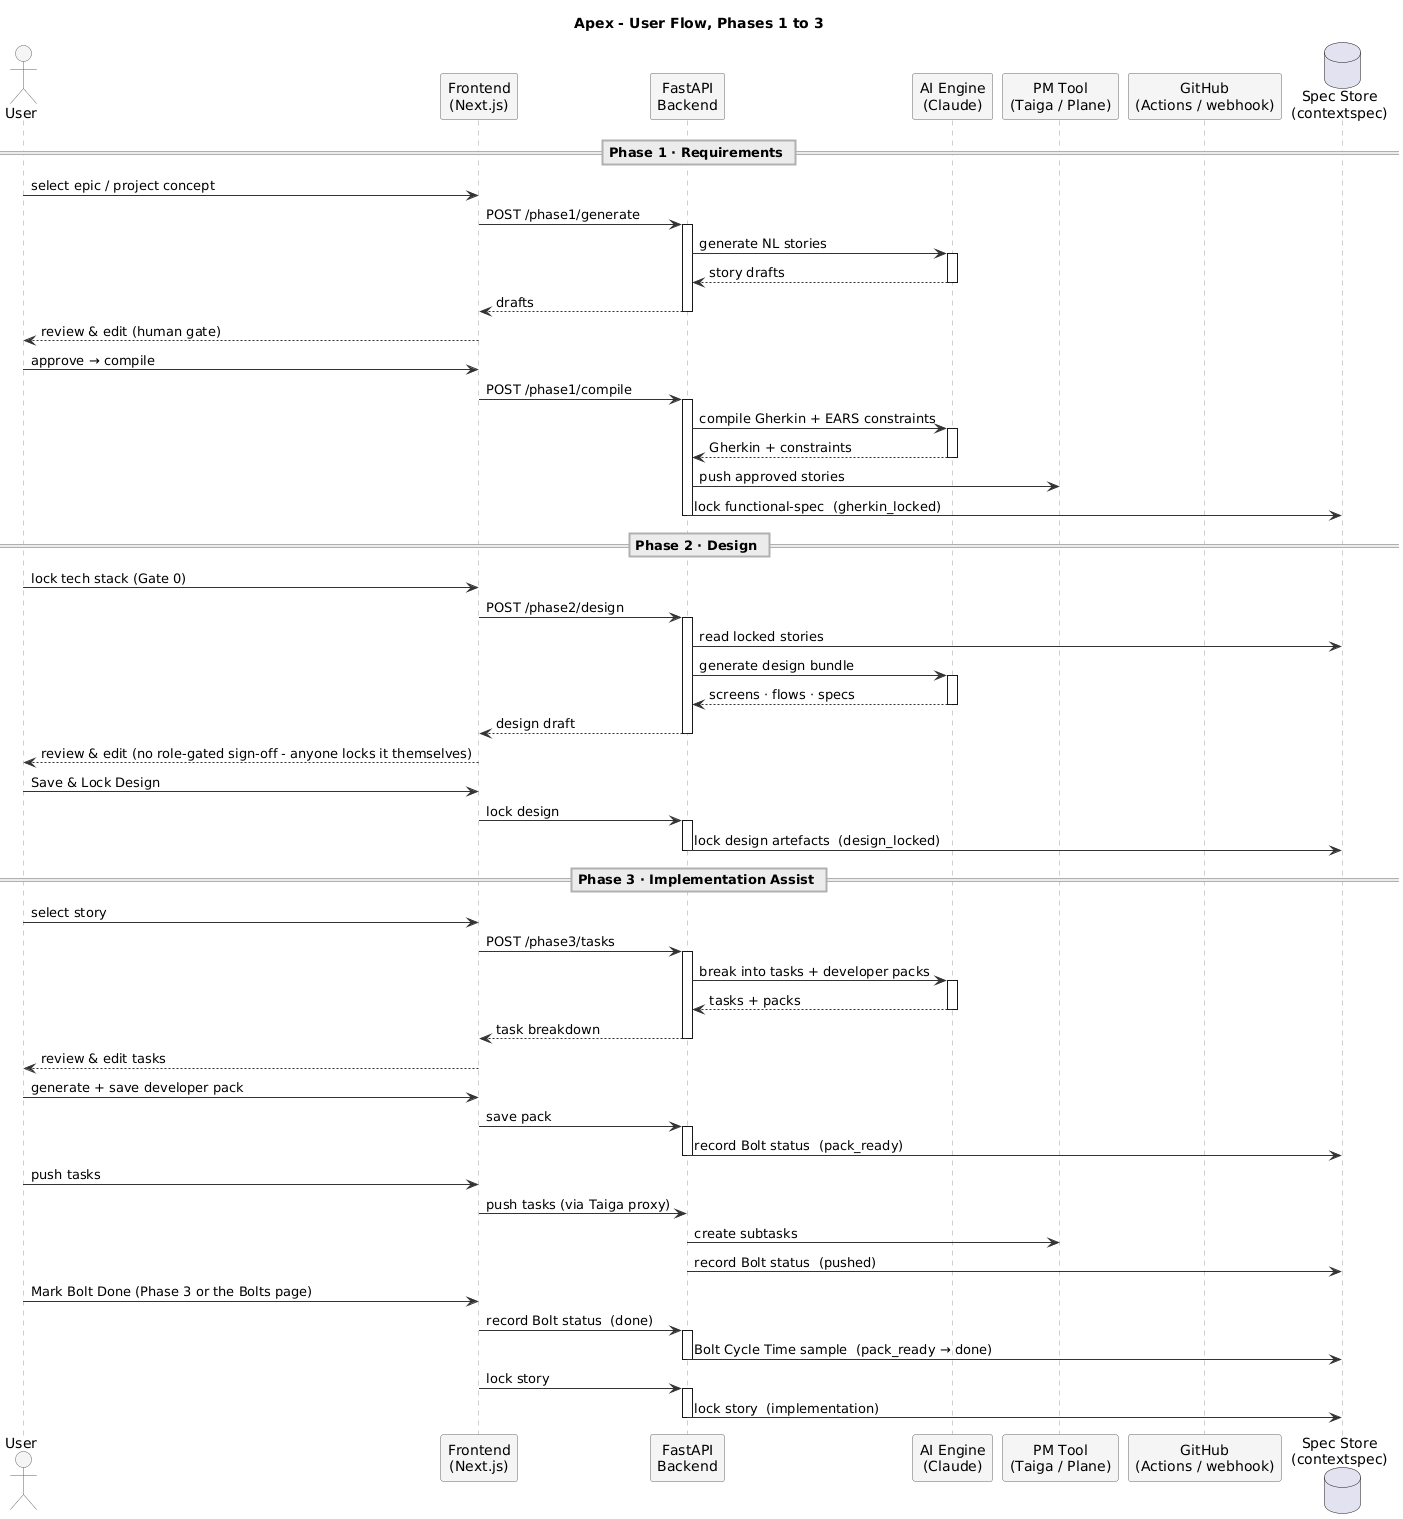
\includegraphics[width=\linewidth]{./Images/user-flow-a.png}
    \caption[A representative walk through Apex, Phases 1 to 3]{A representative walk through Apex, Phases 1 to 3. The figure is split across two pages for legibility; what it is meant to show is that every phase terminates in a write to the specification store and a human acceptance, so no phase can be exited by generation alone.}
    \label{fig:apex_userflow}
\end{figure}

Four of those rows deserve emphasis because they are the ones that answer \ac{DRQ}3 rather than merely illustrating it.

The \textbf{Bolt Cycle Time} row is the clearest instance of a proxy being mistaken for the construct. The framework defines the metric at task level precisely because a story-level measurement conflates execution with the queueing, review and gate transitions surrounding it. The first implementation measured story-level gate transitions and displayed the result under the framework's own name for the task-level quantity, which is exactly the substitution the framework warns against elsewhere. It was corrected, but the fact that it happened at all is evidence for a general point: a construct can be implemented, displayed and believed while measuring something else, and only comparing the implementation against the written definition catches it.

\begin{figure}[htbp]
    \centering
    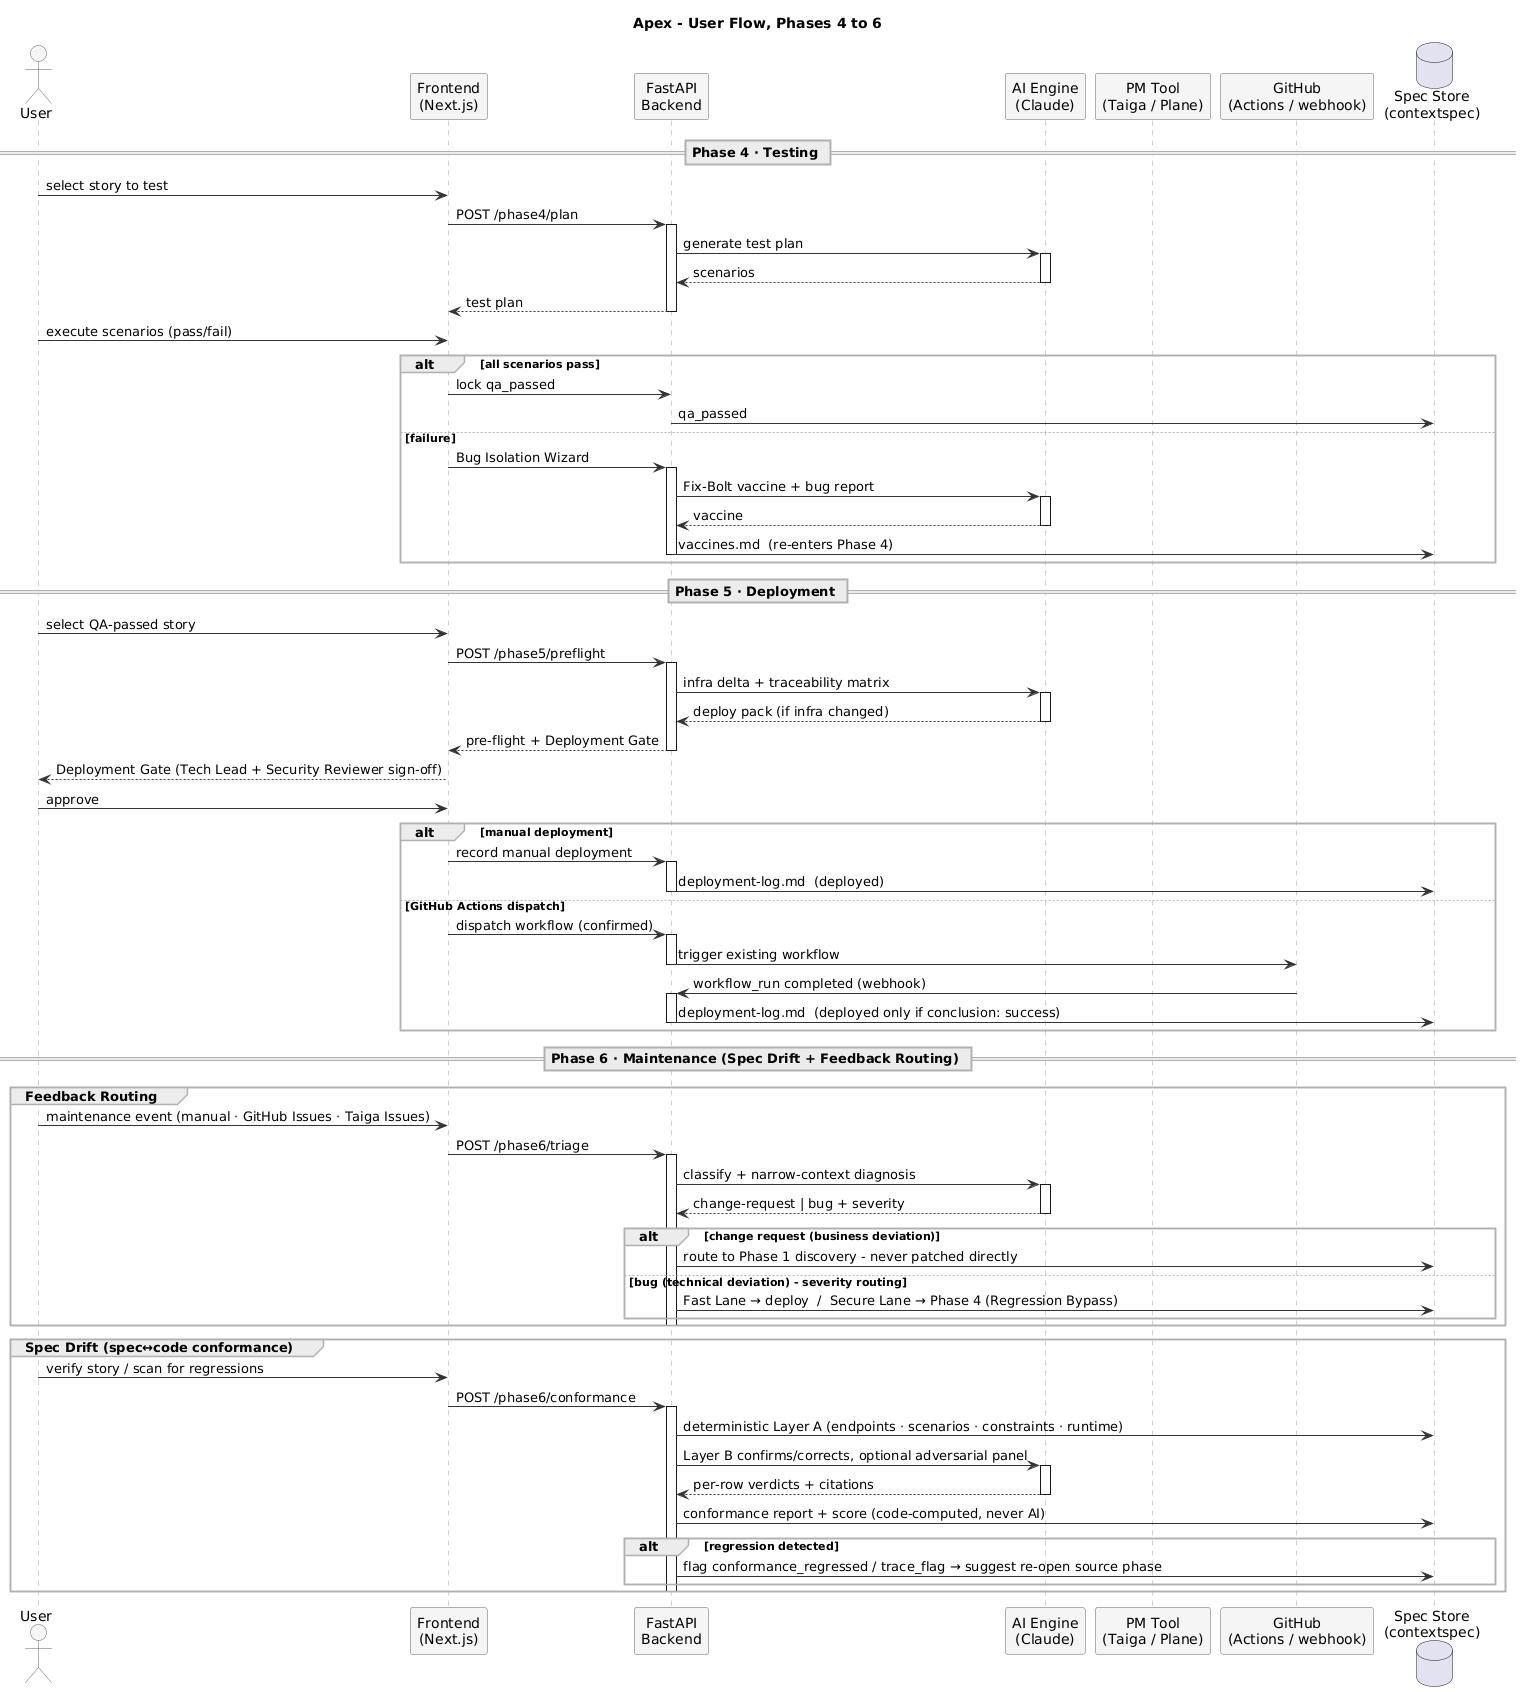
\includegraphics[width=\linewidth]{./Images/user-flow-b.png}
    \caption[A representative walk through Apex, Phases 4 to 6]{The same walk, Phases 4 to 6, continuing \Cref{fig:apex_userflow}. Note the loop-backs out of Testing and out of Maintenance: neither returns to an undefined state, and each re-enters a named phase whose gate then applies in full.}
    \label{fig:apex_userflow_b}
\end{figure}

The \textbf{Context Traceability Rate} row corrects this chapter's own earlier account rather than reporting a later change to the system: the metric had already been computed as an aggregate over deployed stories since June 2026, so the original claim that no aggregate was computed was simply wrong. The error makes the same point \Cref{sec:apex_qa} makes about an unverified self-report: a claim about the system's state is not evidence of that state until it is checked against the code. The strengthening the row records closes a separate gap, where a story could show a complete chain while Phase 6 had already flagged it broken.

\textbf{AI Defect Escape Rate} is realised only as a proxy. The system still cannot observe a production defect directly or attribute one to generated logic, the limitation \Cref{sec:apex_limitations} states and which remains true. The project-management tool already in use carries a usable signal, added in September 2026, that the row describes: reported, linked, post-deployment defects rather than defects in general. That the construct resisted the system's strongest form of observation and was still operationalised at a weaker one worth having is the distinction \Cref{sec:apex_framework_mapping}'s three-outcome taxonomy exists to keep visible, applied here to itself.

\textbf{Spec-drift detection} is the construct that resisted implementation most instructively, and remains only partly resisted. The framework assumes the specification is scoped per story, which is what makes an amendment attributable; the technical specification did not meet that assumption, and the cascade the row records is the consequence. Removing it was the right call, but the finding is not that the feature was hard: it is that a framework construct silently depends on a granularity assumption the framework never states explicitly, and the instantiation is what exposed the omission. That is formative evaluation feeding back into the method, and it is recorded in \Cref{sec:apex_history} as such. The functional specification, unlike the technical specification, already meets that assumption, since each scenario is written under its own story's heading and carries a stable identifier naming that story, which is what made the September 2026 revival possible there. The technical specification was not revived the same way, since no equivalent per-item ownership exists anywhere in the system, and inventing one here would trade the original mistake for its mirror image - false precision in place of false breadth.

% #############################################################################
\section{The Governance Analytics Surface}
\label{sec:apex_analytics}

% Mechanism-level companion to the mapping table above. This describes the
% INSTRUMENT, not results: no figures from a live project belong here, because
% Chapter 9 owns reported numbers and Chapter 8 owns the demonstration gate.

\Cref{tab:apex_mapping} records which governance constructs are realised. It does not say how the numbers standing behind them are produced, and that question decides how much weight \Cref{chap:evaluation} can place on any figure it later reports. Apex computes its governance metrics in one backend service that reads the story index and the context files the workflow has already written, and returns the whole set on demand for the project in scope; at the scale these projects reach, tens of stories, the computation is cheap enough to need no caching and therefore no invalidation rule that could go stale. Two properties of that arrangement matter more than the individual formulas. Nothing on the surface is self-reported: no figure is a model's account of its own work and none is typed in by a practitioner, which is the principle \Cref{sec:apex_qa} describes being violated and then repaired in the coverage badge. And the inputs are a byproduct of running the phases rather than the output of a separate instrumentation step, so a project that is simply used produces its own measurement, and one that is abandoned stops producing it rather than continuing to report a figure that is no longer true of anything. Six figures are displayed, and each is described below by what it actually computes.

\textbf{Context Traceability Rate} is the metric whose implementation is least obvious from its definition, and it is treated first for that reason. \Cref{sec:metrics} defines it as the proportion of deployed work whose context chain is complete, the deployed artefact resolving back to a locked technical specification, to the functional specification it derived from, and to the Unit of Work that motivated it. Apex evaluates that as a predicate, story by story, over every story at deployed status, and reports the proportion satisfying it. The three legs are not equally hard. The artefact-to-Unit-of-Work leg is resolved by construction, since every story-index entry is keyed by the project management tool's own story identifier and cannot exist without one. The functional-specification leg is resolved by per-story attribution that already exists, because scenarios are written under their own story's heading and carry identifiers naming that story. The third leg, the artefact resolving to a locked technical specification, is the one that can break after the artefacts first exist, and it is therefore the only one that is not answered by checking for files. A story satisfies it when its functional, test and infrastructure artefacts are all present, when its identifier is actually found in the deployment log rather than merely claimed as deployed in the index, and when neither of two break detectors is set: an unresolved backward-trace flag, meaning a downstream failure has been pointed at an earlier phase and not yet answered, and an unacknowledged conformance regression, meaning code has since drifted from the specification it was locked against. Either flag zeroes the story even with every artefact file present, because presence is not resolution. A completed verification record then gates the remainder, read from the index where it has been mirrored and from the file itself for indexes written before that mirror existed.

What the metric declines to do is part of its definition. It does not attempt to attribute a deployed story back to particular endpoints or entities within the technical specification, because that ownership does not exist anywhere in the system, for exactly the reason \Cref{sec:apex_framework_mapping} gives for not reviving spec-drift detection there. Claiming to resolve it would substitute fabricated precision for the fabricated breadth already rejected, which is a worse trade rather than a better one. The presence of the technical specification together with the two break detectors is what is honestly provable without it, and the rate should be read as measuring that and no more.

\textbf{Bolt Cycle Time} is computed per task rather than per story. Each story carries its own map of Bolts, and for every task the elapsed time is taken from the earliest timestamp at which it became ready to work to the earliest at which it was marked done; the aggregate over all tasks is reported as a median and a ninetieth percentile in hours. The story-level series that was once displayed under this name still exists and is still useful, but it is shown separately and labelled as cycle time per gate transition, so that the quantity conflating execution with queueing and review can no longer be read as the quantity the framework defines. That the two now sit side by side under different names is the residue of the error described above, and keeping both visible is cheaper than trusting that the mistake will not be repeated.

\textbf{Spec Conformance Rate} is not one of the framework's three metrics but an instrument Apex adds from its own Phase 6 conformance check, which scores generated code against the specification it was locked to on a scale of 0 to 100. The rate is the mean of those scores across every story at implementation status or beyond that has a saved conformance report. A story eligible for the check but never checked is excluded from the mean rather than counted as zero, which fixes what the figure means: it answers how sound the checks that were actually run came out, not whether the checks were run. That second question is a real one and is displayed alongside as the count of eligible stories against the count checked, because the mean alone can be high on a project where conformance has barely been exercised, and a reader given only the mean would have no way to see it.

The two defect figures are best read as a pair, because they observe opposite sides of the deployment boundary. \textbf{Fix-Bolts} counts the corrective micro-cycles raised across the project, reported as a total, as the number of distinct stories carrying at least one, and as a mean per story; these are defects caught by quality assurance before a story shipped, so the figure is a pre-deployment signal and rises when the gate is working rather than when it is failing. \textbf{AI Defect Escape Rate}, whose status as a proxy is argued above and whose limits \Cref{sec:apex_limitations} states, is the post-deployment counterpart: the proportion of deployed stories carrying at least one maintenance item in the project management tool that is classified as a confirmed bug, linked to that story, and dated after that story's own deployment. The classification filter is load-bearing rather than defensive. One supported tool has no issue resource distinct from ordinary work items, so an unfiltered import would count planned work as escaped defects and inflate the rate on precisely the projects that had done the most subsequent work.

\textbf{Stories Tracked} is the plainest of the six, the count of entries in the story index with the deployed subset given beneath it, and it is displayed because the other five are proportions or aggregates that say little until their denominator is visible. A traceability rate over a handful of deployed stories and the same rate over several dozen are not the same claim, and putting the count on the same surface is what stops them being read as one.

A structural distinction runs through the six. Bolt Cycle Time, Context Traceability Rate, Spec Conformance Rate and Stories Tracked are computed entirely from state Apex itself writes while the phases are being worked, so their inputs cannot be absent unless the work itself was absent. The two defect figures depend on issue data owned by the connected project management tool, which Apex reads but does not control and cannot complete. That is why their caveats are sharper, and it is the same boundary \Cref{sec:apex_limitations} draws between what passes through the system and what does not, expressed here as a property of the instrument rather than of the framework. The surface is an instrument and nothing in this chapter reports readings from it; the figures it produces on a real project are \Cref{chap:evaluation}'s to state, under the conditions stated there.

% #############################################################################
\section{Design History and Practitioner Feedback}
\label{sec:apex_history}

% Formative evaluation feeding back into design, not a changelog. Each entry is
% observation, change, rationale, and the framework-level changes are marked.

Feedback gathered while building Apex changed the framework, not only the tool. Recording that path is what makes the \ac{DSRM} iteration explicit rather than implied, and it is reported as observation, change and rationale rather than as a list of releases. Changes made and later reverted are included, because a reverted change is evidence about the design.

Two changes were framework-level and are the clearest evidence that evaluation fed back into the method. The first was the \textbf{removal of a role}: an earlier DevOps Alliance, external to the team and holding deployment approval and infrastructure-security review, was removed once feedback showed a role defined only by what it supervises goes unstaffed, its responsibilities reassigned to whoever performs the deployment (\Cref{sec:roles} argues the rationale in full). What matters here is that the change originated in observation of use rather than in analysis.

The second was the \textbf{demotion of a mandatory step}. Phase 2 originally required a separate sign-off from named design and technical leads before design could be locked. The same observation applied: role-gating a gate presumes a staffed organisation, and on a solo project it either blocks the work or is satisfied by the same person twice, which teaches the practitioner that gates are ceremonial. The step was removed and the gate redefined against recorded evidence rather than against a second signature, which is the form it takes in \Cref{tab:gates}. The framework's position in \Cref{sec:roles} on where a gate's value lies is a direct consequence of this iteration.

Three tool-level changes are worth recording for the same reason. A \textbf{design-conflict detector} was built, then found to flag conflicts that were not conflicts, since two stories in the same epic legitimately share files; it was narrowed to cross-epic file overlap and endpoint collision, and later removed entirely. \textbf{Spec-drift flagging} was built, cascaded as described in \Cref{sec:apex_framework_mapping}, and was removed while its underlying audit trail was kept. An \textbf{authentication flow} for one design integration was built, then reverted for requiring an operator-registered application and a backend-held client secret, incompatible with the tool's zero-configuration setup.

The nature of that feedback bears on how much weight the design history can carry. It came from five practitioners consulted individually during construction, one of whom was consulted a second time after the framework had been substantially revised in response to the first round. The sessions were informal: no interview guide, no fixed question set, no recording, and no demographic data collected. Feedback was captured in the author's own contemporaneous notes as discrete items, each associated with the person who raised it, which is how the changes above are traceable. Participants are not identified and no table of dates or profiles is given, because the sessions were not conducted under any expectation of being reported that way. The record is therefore a participant's notes rather than an independent transcript, and it carries the selection that implies: an item the author did not think worth writing down at the time is not in it.

The limit that follows is a real one, and it belongs here rather than in \Cref{chap:evaluation}. Because each item is attributable, \emph{what} was raised and \emph{what} changed in response are both verifiable against the codebase and the framework document. What cannot be recovered is how strongly any item was held, whether an observation was one person's reaction or a view several would have shared had they been asked, and what the practitioners who did not raise a given point thought of it. The design history is therefore evidence that the method was revised in response to use, which is the \ac{DSRM} claim it is offered for, and it is not evidence about the distribution or strength of practitioner opinion. Three of the five practitioners consulted here later also contributed, separately and with their own consent for that use, to the semi-structured interviews reported in \Cref{sec:interviews}; the two sections draw different material from some of the same individuals, and an item appears in only one place. What the structured interviews add is exactly what this section cannot supply: a written guide, a stated (if under-target) participant profile, and a thematic analysis method applied consistently rather than notes kept only where a design change followed.

The second round is worth isolating, because it produced the sharpest challenge the framework received and the one that changed the shape of this dissertation rather than the shape of the tool. Its substance was that the work was being presented as a product and would therefore be judged as one, against the question of what it offers that a general-purpose coding agent does not; that the scientific questions, why this framework rather than another and how it maps to a given organisation, were being left implicit; and that the correspondence to the published models it draws on should be stated step by step rather than asserted. The response is distributed across three chapters rather than confined to a change log: \Cref{sec:apex_purpose} answers the coding-agent question directly, \Cref{sec:alternatives} engages four named alternatives rather than defending the design in the abstract, \Cref{sec:phases} argues the two points of divergence from its closest published precedent instead of claiming a one-to-one mapping, and \Cref{chap:demonstration} adopts the reframing that the instantiation is itself a demonstration of the method. That a single round of feedback is traceable into four locations of the final document is the clearest evidence available that this was formative evaluation rather than consultation after the fact, and it is reported here in full rather than split with \Cref{sec:interviews} because its effect was on the framework's construction rather than on the distribution of practitioner opinion.

A sixth, later consultation is not part of the five above. An Agile Coach was given a live presentation of the framework and a demonstration of Apex; the reaction, and the two open gaps it named in the tool's interface and in the coach's own organisation's AI governance, are reported in full in \Cref{sec:interviews} as this study's Agile-expert interview. It shares the limits stated for the five practitioners above, and is separated from them because it took place later, checked the demonstration argument rather than shaping the framework during construction, and produced no traceable change to either the framework or the tool.

% #############################################################################
\section{Quality Assurance of the Implementation}
\label{sec:apex_qa}

% Proportionate. This establishes the demonstration platform is sound; it is
% not the contribution.

Testing is layered by what each layer can catch: at the time of writing the backend carries roughly 1,638 tests, the frontend roughly 318 unit tests, and there are 24 end-to-end test cases across 12 specifications, a snapshot of a codebase that continues to change.

Testing also surfaced defects with methodological significance. A section-parsing routine truncated a live project's technical specification part-way through because it anchored on headings the model itself also emits. An automation step once marked a story's quality gate as passed with no verification behind it, and the deployment step trusted that result rather than checking it. And the identity anchor determining which tenant a request belongs to, along with an integrated tool's listing endpoint, each leaked across project boundaries before being corrected. A coverage badge reported the model's own claim about which scenarios it had covered, at face value; it is now reconciled server-side against the parsed specification, and a claimed scenario that does not match a real one is dropped rather than displayed.

% #############################################################################
\section{Limitations of the Implementation}
\label{sec:apex_limitations}

The limitations of Apex as a system must be separated from the limitations of the framework as a methodology, because conflating them would let a defect in one be read as a refutation of the other.

Two are limitations of the system. The single-writer fallback path, which most deployments would run, is a real ceiling rather than a theoretical one (\Cref{sec:apex_architecture}). And Apex observes only what passes through it: it can see a story's specification chain, and, once a defect is reported through the project-management tool and linked to a story, a proxy signal that a deployment shipped a fault - but it cannot observe a defect never reported there, or attribute one to generated logic specifically.

Two are limitations that belong to the framework and were exposed by trying to build it, and both remain open even after the September 2026 work reported above. \textbf{AI Defect Escape Rate, at the observation point the framework's own definition presumes, is not instantiable by this class of system}: nothing in the framework says who owns production telemetry for generated logic specifically, and a tool sitting above a project-management board has no access to it regardless of who does; what is instantiable is the weaker proxy described in \Cref{sec:apex_framework_mapping}. \textbf{Spec-drift detection presumes a granularity the framework does not state}, namely a per-story rather than a per-project specification, and the instantiation revealed the omission by failing on it; it now holds for the functional specification and remains open for the technical one. Both are carried into \Cref{chap:evaluation} as findings rather than as defects to be excused.

The two proxies differ in kind, and \Cref{tab:apex_mapping} names both as proxies rather than presenting either as the construct itself: Bolt Cycle Time was one briefly and by accident, while AI Defect Escape Rate is one by design from the outset. A substitution left unnamed is indistinguishable from the thing it substitutes for.
